\documentclass{subfiles}
\begin{document}
\begin{wrapfigure}[16]{l}{0.425\textwidth}
    \centering
    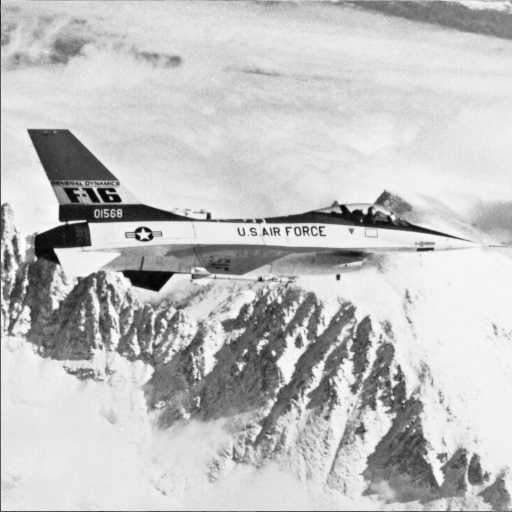
\includegraphics[scale = 0.325]{Images/Airplane/Stretched Airplane.png}
    \caption{Stretching di \emph{Figura \ref{fig:4.8}}.}
    \label{fig:8.1}
\end{wrapfigure}
Per prima cosa, si parta dal considerare \emph{Figura \ref{fig:8.1}}, questa è stata ``stretchata'': ossia considerando la scala di grigi dell'immagine,
quest'ultima è stata modificata così da sfruttare l'intera scala.

\begin{Remark*}
    lo stretching di immagini è effettuabile unicamente se, considerata la scala di grigi,
    questa presenta come valore di massimo (minimo rispettivamente) un valore diverso da 255 (0 per il minimo).
\end{Remark*}

\noindent Sebbene in apparenza uguale a \emph{Figura \ref{fig:4.8}, Figura \ref{fig:8.1}} differisce totalmente.
Tale differenza, che ad un occhio inesperto risulta appena percettibile, è più facilmente osservabile se si considera l'istogramma.
Da questi, in \emph{Figura \ref{fig:8.2}.b}, si notano delle spaccature equidistanti, dovute appunto allo stretching dell'immagine.

\begin{Remark*}
    le spaccature in sè nell'istogramma non sono indicative, esistono infatti immagini non stretchate che presentano spaccature;
    ad esserlo è il fatto che queste sono equidistanti.
\end{Remark*}

\noindent Considerando dunque gli istogrammi, sia di \emph{Figura \ref{fig:4.8} \emph{che} Figura \ref{fig:8.1}}, si ottiene quanto riportato in \emph{Figura \ref{fig:8.2}}.
\subfile{../Figure/Figure 8.2 - Confronto istogrammi.tex}

Per quanto riguarda i codici MATLAB utilizzato per lo stretching, questi è di seguito riportato.
\begin{center}
    \begin{lstlisting}[language = MATLAB]
        function out = stretch(img)
            img = double(img);
            minI = min(img(:));
            maxI = max(img(:));
            out = uint8(round(255*(double(img) - minI)/(maxI - minI)));
    \end{lstlisting}
\end{center}

Analizzando brevemente il codice, quanto sopra definisce una nuova funzione \lstinline[language = MATLAB]{stretch},
evidenziata dalla keyword \lstinline[language = MATLAB]{function}. Nel caso particolare, questa richiede una variabile a cui assegnare il risultato quando chiamata.
\end{document}